\part{Theory}
\chapter{Crystal structure analysis}
\label{ch:csa}
Chapter \ref{ch:csa} is adopted from the textbooks ``Kristallstrukturanalyse''  by W. Massa \cite{massa} and ``Einführung in die Röntgenfeinstrukturanalyse'' by H. Krischner \cite{krischner}. 
\section{Definitions}
A solid that contains atoms, ions or molecules which are arranged in a periodic pattern along the three dimensions of space is described as a crystal. For an arbitrary point picked in the crystal there are infinitely many points with identical surroundings. This is called periodicity. The crystal  can be considered infinitely extended in three dimensions. It can be seen as a lattice with a three dimensional array of points (lattice points). These points may not be considered as the ions or atoms in the crystal. If an atom is positioned on a lattice point, then the same atoms are at every lattice point in the crystal. \cite{massa}

 
\section{Bravais lattice}

7 crystal systems can be determined from a variation of the lattice parameters a, b, c and the angles $\alpha, \beta, \gamma$. Together with four types of centered cells (primitive (P), body-centered (I), face-centered (F) and base-centered (B)) 14 Bravais lattice types can be defined. \cite{bravais} For their determination the entire symmetry of the crystal should be contained in the smallest  unit of the cell. In table \ref{tab:cryssys} the crystal systems are listed.

\renewcommand{\arraystretch}{1.2}
\begin{table}[!htpb]
\centering
\captionabove{Crystal systems with their types of centered cell}
\begin{tabular}{|l|l|l|l|}
\hline
\textbf{Crystal system} & \textbf{Parameter} & \textbf{Angles} & \textbf{centered cell}\\
\hline
triclinic & $a\neq b\neq c$ & $\alpha\neq\beta\neq\gamma\neq 90^\circ$ & P\\
\hline
monoclinic & $a\neq b\neq c$ & $\alpha=\gamma=90^\circ \beta>90^\circ$ & P, B\\
\hline
orthorohmbic(cuboid) & $a\neq b\neq c$ & $\alpha=\beta=\gamma= 90^\circ$ & P, F, I, B \\
\hline
tetragonal & $a= b\neq c$ & $\alpha=\beta=\gamma= 90^\circ$ & P, I \\
\hline
hexagonal & $a= b\neq c$ & $\alpha=\beta= 90^\circ \gamma=120^\circ$ & P\\
\hline
trigonal (rhomboedric) & $a= b= c$ & $\alpha=\beta=\gamma\neq 90^\circ$ & P\\
\hline
cubic & $a= b = c$ & $\alpha=\beta=\gamma= 90^\circ$ & P, F, I\\ 
\hline
\end{tabular}
\label{tab:cryssys}
\end{table}

 \section{Diffraction}
 Electromagnetic waves can  interact with one-dimensional lattices. When monochromatic light (wavelength $\lambda$)  irradiates an optical grating (period d, which is the distance between two adjacent lines) and they are in the same order of magnitude, diffraction can occur. When a point of the lattice is struck with light, becoming a spherical wave of the same wavelength, it is called elastic scattering. The waves interfere with each other depending on the angle $\theta$ of observation and  the difference of the travelled path lengths by waves of the two adjacent points (optical retardation $\Delta$). Constructive interference can occur when $\Delta$ is an integer multiple of the wavelegth $\theta$. If all scattered waves in phase reinforce one another it leads to an observable diffracted beam. Destructive interferences between scattered waves can be observed if $\Delta$ is a half integer of $\theta$ and annulles them completely. In all other cases, where the values are between constructive and destructive interference, the lattice points can be grouped in pairs and be separated by one or more lattice points. These scattered waves are out of phase and cancel each other out. The intensity of the angles which meet the requirement of constructive interference exactly will be observed, the others will not.
 
 \begin{figure}[htpb!]
 \centering
 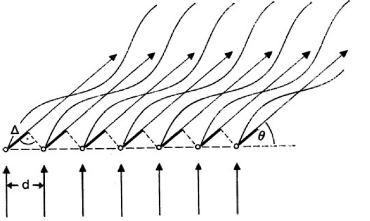
\includegraphics[width=0.7\textwidth]{figures/diffraction.png}
 \caption{Diffraction on a one dimensional lattice \cite{massa}}
 \label{fig:dif}
 \end{figure}
 
 \section{Bragg's Law}
In order to obtain diffraction, X-rays are  used since their wavelengths have the same order of magnitude as the inter-atomic distances in crystals, 1 \AA or 10$^{-10}$ m.  For three dimensional lattices, the one dimensional diffraction has to be adapted. The reflection of X-rays on lattice planes can be treated as diffraction. \cite{bragg} Only if constructive interference occurs (retardation is whole multiple of the wavelength) the conditions are fullfilled and Bragg's Law can  be derived (eq. \ref{eq:bragg}).  


\begin{figure}[htpb!]
\centering
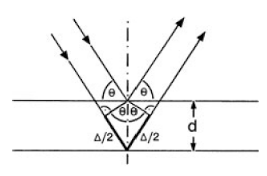
\includegraphics{figures/bragg.png}
\caption{Derivation of Bragg's Law \cite{massa}}
\label{fig:bragg}
\end{figure}


\begin{equation}
\begin{split}
2d sin(\theta) = n\lambda\\
 n=1,2,3,...
\label{eq:bragg}
\end{split}
\end{equation}



\section{hkl indices}
 All of the lattice planes contain lattice points and for each lattice plane there is a set of parallel and equidistant planes. Each lattice point lies on one plane. 
 For orientation of the planes there are the Miller Indices hkl. For the determination of the Miller indices for a set of planes, the plane nearest to the unit cell's origin (don't contain the origin)  is picked. This plane intersects the a-, b- and c-axes with the distances 1/h, 1/k and 1/l from the origin  measured in the axis lengths' units. 1/h, 1/k and 1/l can be represented as fractions, because they are rational numbers. The lattice planes can be denoted in parentheses (hkl) and hkl is used for the corresponding reflection. For parallel planes (to an axis) the intersection point lies at infinity and the Miller index is zero. For each set of lattice planes (hkl) with the characteristic distance d there is an unique angle $\theta$ for each diffraction order n at which reflection can be observed. (see Bragg's Law, eq. \ref{eq:bragg}). Each Miller index can be multiplied by n to determine the reflection at a lattice point.
 
 

 

 \section{Solution of Bragg's formula}
 To calculate the diffraction angle $\theta$ the distance of the corresponding lattice plane must be known. The distance d depends on the Miller indices (hkl) and the geometry of the lattice. The distance can be a square number (d$^2$) if different crystal systems are used. If Bragg's equation \ref{eq:bragg} is squared and d$^2$ is substituted, a quadratic Braggs' law is formed. It can be used to calculate $\theta$ from the Miller indices if the unit cell is known.
 
 
\section{Reciprocal lattice}
Each reflection is equivalent to a specific set of lattice planes. These sets are described by a vector d whose direction is vertical to the planes. Its length is equal to the distance between two adjoining planes. The endpoint of the corresponding vector d represents a lattice plane. For higher diffraction angles the length of d is shorter, which can be a drawback. Also hkl cannot be used to determine the direction of d. A new coordination system can help prevent these difficulties. It is spanned by the three base vectors a*, b* and c* and represents each plane (hkl) and each reflection hkl as the point ha*+ kb* + lc*. The reciprocal lattice is formed with the points of all possible coordinations of the indices, which are whole numbers. The original lattice is called the crystal lattice to distinguish the two.  The reciprocal base vectors are formed from the real base vectors in eq. \ref{eq:recv}, where each numerator is the vector product of two real base vectors and (abc) is the triple product equal to the volume of the real unit cell.
\begin{equation}
\begin{split}
a* =b x c/(abc)\\
b* = c x a/(abc)\\
c* = a x b/(abc)\\
\end{split}
\label{eq:recv}
\end{equation} 

 While in orthogonal crystal systems each reciprocal base vector is parallel to its counterpart, this is not true for systems with  oblique angles. Eq. \ref{eq:recv} suggests that every unit vector in reciprocal space is perpedicular to a plane in real space and vice versa. 

 \begin{figure}[htpb!]
\centering
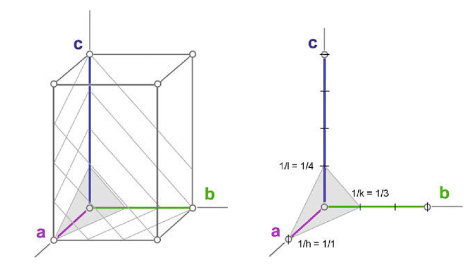
\includegraphics{figures/hkl-indices.png}
\caption{Definition of the hkl-indices through reciprocal axis intercept \cite{massa}}
\label{fig:hkl}
\end{figure}

\section{Intensity of diffracted X-rays}
With the knowledge of the geometry of the crystal lattice (the metric) the angles of all possible reflections can be determined. This is used in powder and single crystal measurements. The intensities of the reflections contain information about type and location of atoms in the unit cell. They can be measured absolute or relative. Absolute values are difficult to determine but relative values can be calculated and then be scaled to absolute values. How the atoms are arranged in the crystal can be calculated with these values. All factors should be known because they affect the intensities.

\section{Atomic scattering factor and temperature factor}
Up to now it was considered that X-ray scattering takes place at the points of the point lattice . In reality scattering occurs at the electrons or ions of atoms and crystals.  It was established that the radius of an electron shell has the same magnitude as the X-ray wavelength, but punctual scattering centers are not in the same range. Therefore  rays that are scattered at different positions in the electron shell have a phase difference. This leads to a weakening of the intensities which depends on the form of the shell and on the diffraction angle.  The scattering factors are scaled in a way that their values at an angle of zero are equal to the corresponding atomic number. \\
Atoms, depending on atom mass, chemical environment and temperature, oscillate about their equilibrium positions. X-ray beams consists of short radiation flashes that are approximately $10^{-18}$ s long. This is much shorter than the period of a thermal oscillation, lasting for $10^{-14}$ s. Because of this a specific atom can appear at slightly different locations during measurement. The result is a phase difference which increases with larger amplitudes (u) and smaller distances of the lattice planes, i. e. larger diffraction angles. This additional weakening of the scattering factors f is taken into account by multiplying the scattering factors with an e-function. At the beginning of a calculation the oscillations are assumed to be isotropic (see equation \ref{eq:os}). Substituting d in accordance with Bragg's Law eq. \ref{eq:bragg} and absorbing some constants in the Debye-Waller-factor B \cite{debye}\cite{waller} result in eq. \ref{eqdwfb}.

\begin{equation}
f' = f \cdot e^{-2\pi^2 \frac{u^2}{d^2}}
\label{eq:os}
\end{equation}



\begin{equation}
f' = f \cdot e^{-B\frac {sin^2 \theta}{\lambda^2}}
\label{eqdwfb}
\end{equation}

This affects the determination of lighter atoms, which have both low scattering factors and high amplitudes, due to their low mass. The crystals should be cooled when they are measured because of these reasons. When refining the crystal structure, oscillations are usually considered to be anisotropic with the exception of H-atoms. The displacement is now described by a tensor, represented by a symmetric 3x3 matrix with six independent factors,  U$_{11}$,  U$_{12}$,  U$_{13}$,  U$_{22}$,  U$_{23}$,  and U$_{33}$. By visualizing it as a thermal ellipsoid with three axes the corresponding atom can be found within the ellipsoid with 50\% probability. 


\begin{equation}
f'=f  \cdot e^{-2\pi^2(U_{11}h^2a^{*2}+U_{22}k^2b^*2+U_{33}l^2c^*2+2U_{23}klb^*c^* +2U_{13}hla^*c^*+2U_{12}hka^*b^*)}
\end{equation}


\section{Structure factor}

A reference point in the crystal is selected and all the other points whose surrounding are identical to that selected one  are determined in order to obtain the point lattice of the crystal. If a different reference point is picked, the same lattice is given, only shifted by the translation vector. This vector equals the difference of the spatial positioning between the first and second reference point. The same lattice applies to every atom in the unit cell, the chosen origin is the only difference. The crystal in fig. \ref{fig:pl} needs to be adjusted so that the lattice plane is at an appopriate angle $\theta$ with the X-ray beam. Then the waves of all type 1 atoms are in phase with each other.
\begin{figure}[htpb!]
\centering
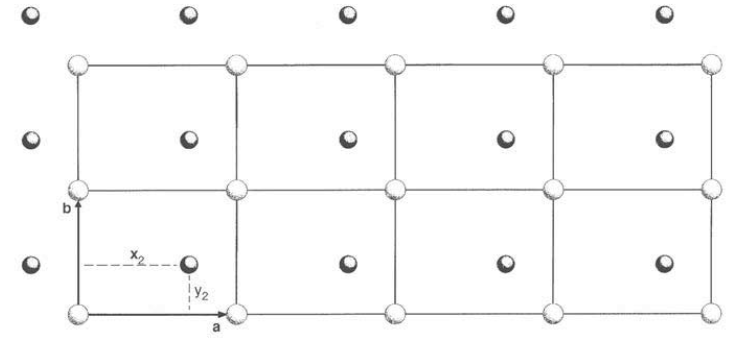
\includegraphics[width=1\textwidth]{figures/pointlattice.png}
\caption{2D- structure with two types of atoms \cite{massa} }
\label{fig:pl}
\end{figure}



 Waves generated by atoms of type 2 are also in phase with each other, because $\theta$ is not changed when the lattice is shifted . Since the lattice is translated a phase difference between the two diffracted rays exists. This depends on the relative position of the two atom types and on the selected lattice plane. Scattering factors are extended by a phase information, by multiplicating an exponential function with an imaginary argument: 




\begin{equation}
F_{hkl}(n) = f_n \cdot e^{i\phi_n}
\label{eq:hkl}
\end{equation}

For each atom of type n the phase angle $\phi$ expresses the phase difference. Euler's formula is applied to eq. \ref{eq:hkl} and gives an equivalent function with the sin und cos terms:

\begin{equation}
F_{hkl}(n)= f_n(cos(\phi_n)+i\cdot sin(\phi_n))
\end{equation}

In order to calculate $\phi_n$  the relative coordinates x$_n$, y$_n$, z$_n$ of atom n in the unit cell and the Miller indices of the lattice plane are taken into account: 

\begin{equation}
\phi_n = 2\pi(hx_n + ky_n + lz_n)
\end{equation}

For each reflection the diffracted waves of all atoms are added together with regard to their phase differences which leads to the final equation for the structure factor F$_{hkl}$ for a certain reflection hkl:

\begin{equation}
F_{hkl} = \sum_n f_n[cos(2\pi(hx_n + ky_n + lz_n)) + i\cdot sin(2\pi(hx_n + ky_n + lz_n))]
\end{equation}

For crystals belonging to a centro-symmetrical point group - with the origin of the crystal lattice being placed at a center of inversion - the calculation of the structure is reduced to:

\begin{equation}
F_{hkl} = \sum_n f_n cos(2\pi(hx_n + ky_n + lz_n))
\end{equation}

The structure factor cannot be measured directly because it is an imaginary quantity. Its relative intensity is determined and this is proportional to  the absolute value of F$_{hkl}^2$ . The phase angle $\phi$  cannot be obtained directly from the intensities, because it gets lost through the calculation -  this is called the phase problem. If the crystal has an inversion center, the phase problem can be simplified to determining the sign of F$_{hkl}$.

\section{Processing data}
For obtaining structure factors the raw data has to be processed after measurement. First the background signal is substracted and normalized if different periods are measured. The net intensity of each reflection is computed from the total intensity with this method. Intensities of reflections at different angles can be compared among each other when correction factors are applied. For powder diffractometry the multiplicity factor is relevant. This factor takes in consideration  that reflections of symmetry-equivalent lattice planes appear at the same angle in a powder diffractogram. The multiplicity factor normalizes the intensities since different lattice planes may have different numbers of symmetry equivalents. The value of the factor  ranges from 2 to 48 (triclinic to cubic system). The diffraction of X-rays is a reflection at certain planes in the crystal. The reflection angle $\theta$ is not important for the intensity of the fraction of the reflected beam, only if the electric component lies parallel to the plane. The intensity fraction is proportional to cos$^2$(2$\theta$) for radiation whose electric vector oscillates perpendicular to the plane. The polarization facor P makes it possible. Unpolarized X-rays leave the X-ray tube as a 1:1 mixture of rays with parallel and perpendicular electric field vectors to the reflection plane. Between these two extreme cases P is simply the average of the two:

\begin{equation}
P = \frac{(1 + cos^2(2\theta))}{2}
\end{equation}

A reflection is a curve with a certain breadth with its peak located at $\theta$ (Bragg's  angle). If a single crystal is rotated in the diffractometer the lattice planes stay in a reflection position for a period of time. It depends on the value of $\theta$ and is factored in the Lorentz factor L:

\begin{equation}
L = \frac{1}{sin(2\theta)}
\end{equation}

Lorentz and Polarization factor are summarized in the LP-correction:
\begin{equation}
LP=\frac{1+cos^2\theta}{2sin 2 \theta}
\end{equation}

The observed structure factor F$_0$ may be calculated as:
\begin{equation}
F_0=\sqrt {\frac{I}{LP}}
\end{equation}
 The absorption factor must also be taken into account. It affects the relative intensities of diffracted X-rays. While traveling through matter X-rays are weakened by elastic scattering, inelastic scattering and ionization. These absorption effects increase approximately with the fourth potency of the atomic number of the absorbing atom and with the third potency of the wavelength of the X-rays. All effects are summarized in the linear absorption coefficient ($\mu$) and the intensity can be calculated with eq.\ref{eq:lac} (s is the travelled distance of the X-ray beam):

\begin{equation}
I = I_0\cdot exp(-\mu\cdot s)\\
\label{eq:lac}
\end{equation}

From tabulated values for components of the crystal, their mass fraction in the crystal and the density of the crystal $\mu$ can be obtained. Different methods for absorption corrections (for higher $\mu$ values) have been developed, e.g. numeric absorption correction, empiric absorption correction and the DIFABS method \cite{wal83}.

\section{Laue class}
For determination of the space group the Laue class must be derived. Each reflection is a point in the reciprocal lattice. Assigning the intensity to each reflection of its point in reciprocal space yields the intensity-weighted reciprocal lattice. Its point group is the Laue class of the crystal. The Laue class contains a center of inversion (even if the crystal has none) which is the only difference between the space group and the Laue class. The two reflections hkl and h-k-l refer to the same set of lattice planes except they are only irradiated from opposing sites. All Laue groups include two or more point groups and each point group contains several space groups. \\
For reducing the number of possible space groups systematic extinctions can be found. They are absences of reflections whose indices satisfy certain conditions. They show that glide planes, screw axes or centered unit cells can be present in the cell. For crystal systems of high symmetry the space group can be hardly determined. For these cases informaton about physical properties, Patterson symmetry and structure-chemical plausibility is important.  


\section{Direct methods}
These methods attempt to obtain phases of the structure factors directly from measured intensities through mathematical relationships. The original works for these methods  \cite{harker48} found that the presence of symmetry elements gives rise to relations between structure amplitudes and certain pairs of reflection. The assumption that the electron density consists of identical and well-resolved peaks result in the equation \ref{eq:dm} \cite{sayre}:
\begin{equation}
E_{hkl} = C \sum_{h^{'}k^{'}l^{'}}E_{h^{'} k^{'} l^{'}} \cdot E_{h-h^{'} k-k^{'} l-l^{'}}
\label{eq:dm}
\end{equation}

To obtain the normalized structure factor E$_{hkl}$ F$_{hkl}$ is divided by its expectation value. This value can be calculated from the Wilson statistic. \cite{wilson}  Eq.\ref{eq:dm} applies to structures containing just one type of atom but in practice it can also be used for structures with atoms with similar atomic number; e.g. C, N, O, H. Therefore it can be applied for classes of structures that are difficult to solve via Patterson methods.



\section{Patterson method}
For crystals containing only a few heavy elements (which is the case for most metal-organic compounds) the Patterson method can be of use, as it  solves the phase problem.
In the Patterson function P$_{uvw}$, the coefficients are the directly measured F$_0^2$ values. To distinguish the patterson synthesis from a normal F$_0$ Fourier synthesis, the coordinates in Patterson space have the coordinates u, v and w. These 
coordinates are not directly related to atomic coordinates x, y, z, altough they refer to the same axes and unit cell. 
The Patterson function is defined as:
\begin{equation}
P_{uvw}= \frac{1}{V} \sum \limits _{hkl}\left|F_{hkl}\right|^{2} cos(2\pi(hu + kv + lw))
\end{equation}

The Patterson function only include the information  from the intensities, the interatomic vectors, because no phase information is contained in the F$_0^2$ values.  \cite{patterson}\\

Maxima in the function P represent distance vectors between atoms in the unit cell. P is always centrosymmetric since two distance vectors of the same length and opposite direction are associated with each pair of atoms. The intensity of a Patterson peak is simply the product of the atomic number of the two atoms involved. If a crystal contains a few heavy metal atoms, they can easily be identfied by the high intensities of the corresponding peaks. 


